With 100\% infill, 3D printed PLA has a maximum shear stress of 13.6 kpsi. The manipulator applies a load of 13N in the negative y-direction. Without gears in the base differential, the differential support would bear the load on its bearing mounts. \emph{Figure \ref{fig:tbar}} shows the manipulator’s differential support could experience up to 97 kPa or 0.014 kpsi of shear stress, which is less than the maximum shear stress of PLA with 100\% infill. Since some of the manipulator’s mass is supported by the gears, the actual shear experienced by the differential support will be less.

\begin{figure}[htp]
  \center
  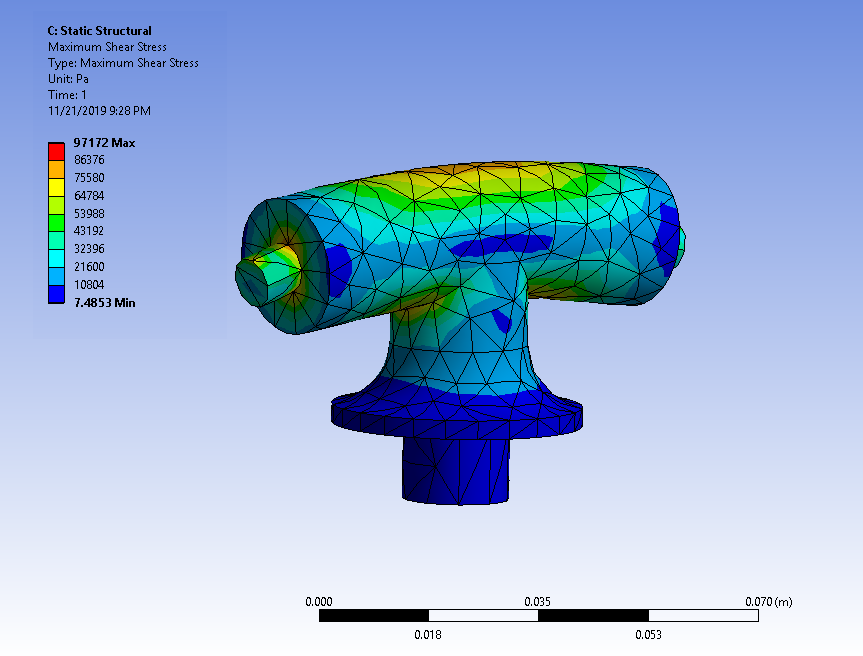
\includegraphics[width=.5\textwidth, frame]{tbar}
  \caption{T-Bar ANSYS FEA}
  \label{fig:tbar}
\end{figure}

To simulate a dynamical loading situation where the manipulator would be under the largest amount of stress, gravitational forces and an outward force (parallel to the arm direction in it's zeroed configuration) were applied to the structure. This situation represents the worst-case loading scenario, such as the manipulator swinging while outstretched. The supports and simulated forces can be seen in the ANSYS image capture shown in \emph{Figure \ref{fig:ansys_forces}}.
\begin{figure}[htp]
  \center
  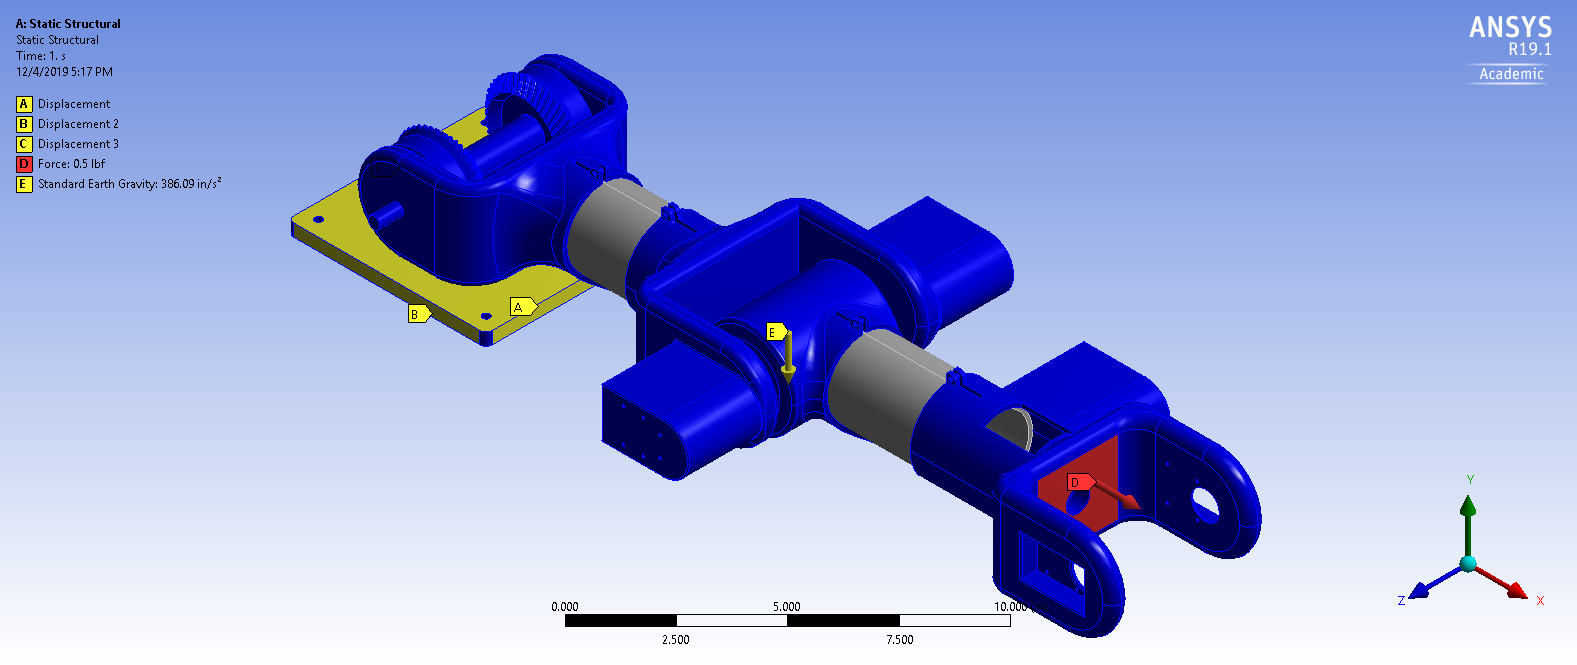
\includegraphics[width=.55\textwidth, frame]{ansys_forces}
  \caption{ANSYS Simulated Forces Image Capture}
  \label{fig:ansys_forces}
\end{figure}
\newpage
As shown in \emph{Figure \ref{fig:ansys_forces}}, the red arrow is the outward force simulating centrifugal forces, the yellow arrow represents gravity acting at the manipulator's center of mass, and the yellow highlighted faces show the fixed support at the base.

The dynamical loadings resulted in a maximum shear stress at the shoulder differential bearing, as seen in \emph{Figure \ref{fig:ansys_full}}; a close-up image of the bearing analysis can be seen in \emph{Figure \ref{fig:ansys_bearing}}.

\begin{figure}[htp]
  \center
  \begin{subfigure}[t]{0.5\textwidth}
  \center
  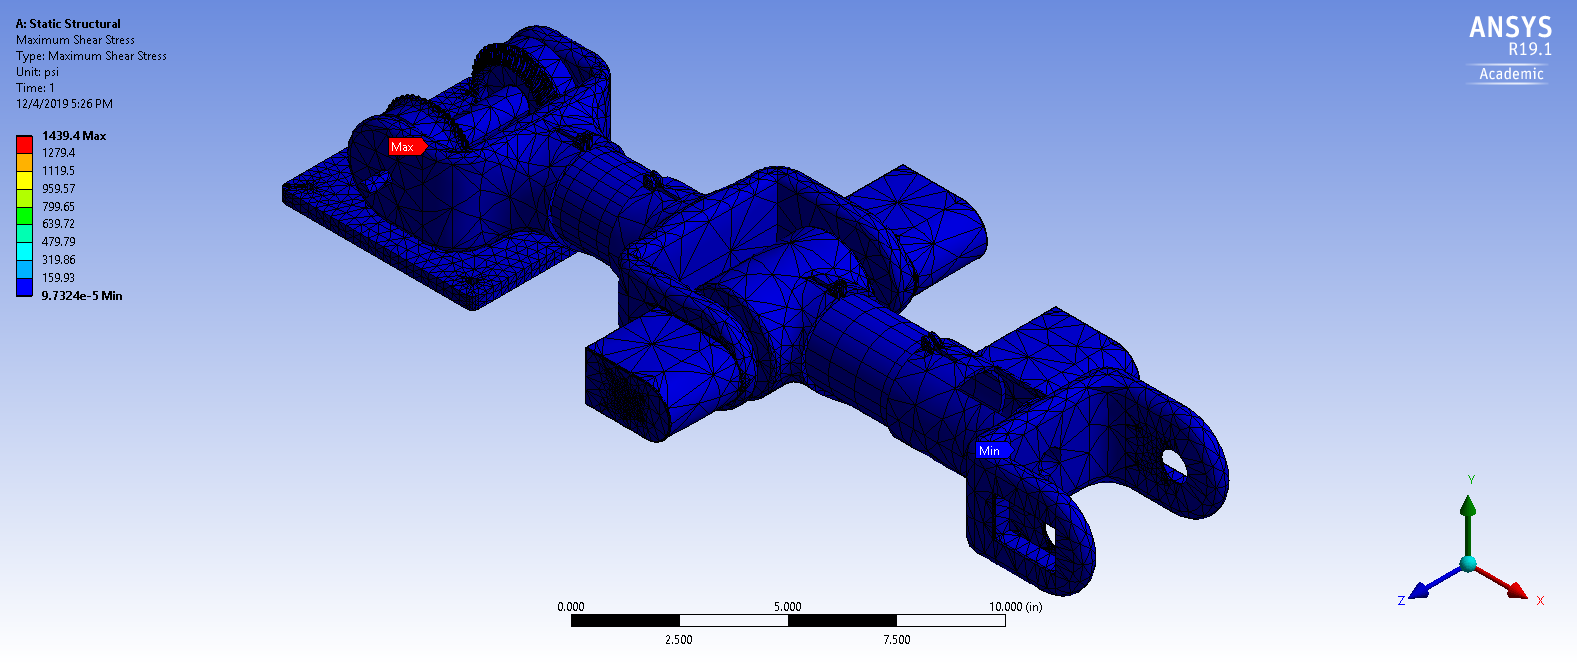
\includegraphics[width=.9\textwidth,frame]{ansys_full}
  \caption{ANSYS Full View of Maximum Shear}
  \label{fig:ansys_full}
\end{subfigure}%
\begin{subfigure}[t]{0.5\textwidth}
  \center
  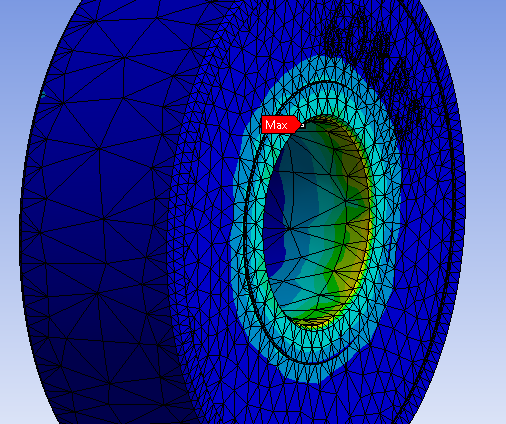
\includegraphics[width=.75\textwidth,frame]{ansys_bearing}
  \caption{ANSYS Bearing Shear Stress Close-up}
  \label{fig:ansys_bearing}
\end{subfigure}
  \caption{ANSYS FEA of Dynamical Loading Scenario}
\end{figure}

To further validate that the structure is capable of handling alternating stresses, a fatigue test was also performed showing the life of the manipulator handles a minimum of 1e6 cycles, as seen in \emph{Figure \ref{fig:ansys_life}}, showing it is unlikely to fail due to material yeilding.

\begin{figure}[htp]
  \center
  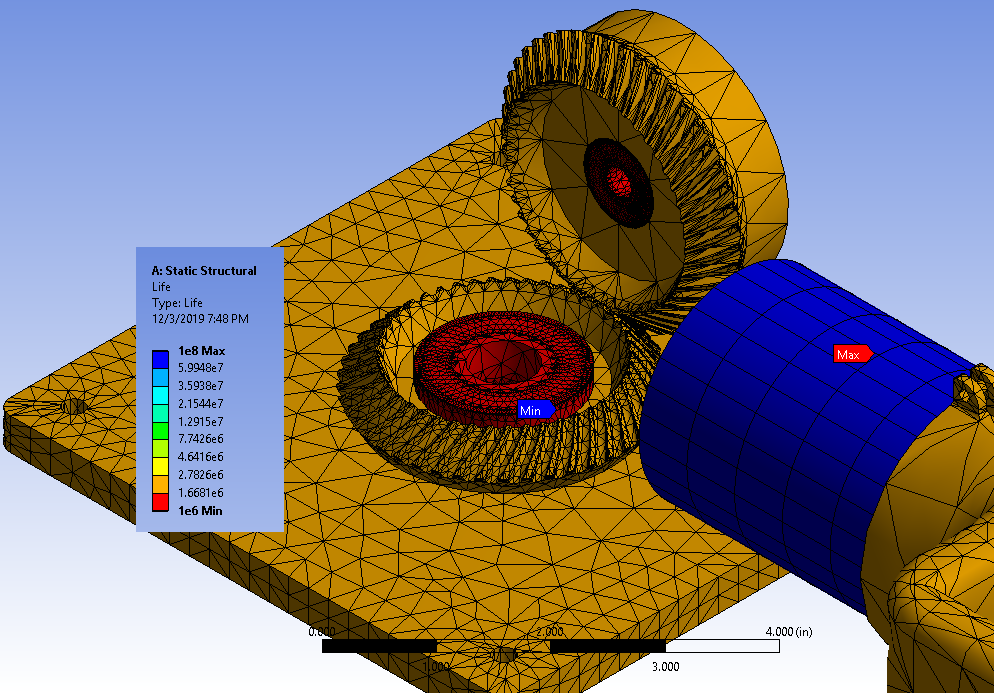
\includegraphics[width=.6\textwidth, frame]{ansys_life}
  \caption{ANSYS Fatigue Test}
  \label{fig:ansys_life}
\end{figure}

As seen in \emph{Figure \ref{fig:ansys_life}}, the lower bearing of the differential drive on the shoulder of the manipulator would be the most likely component to fail under repeating loadings.
